%%%%%%%%%%%%%%%%%%%%%%%%%%%%%%%%%%%%%%%%%%%%%%%%%%%%%%%%%%%%%%%%%%%%%%%%%%
% Output voltage u2 for M3C with RLE-Load
%%%%%%%%%%%%%%%%%%%%%%%%%%%%%%%%%%%%%%%%%%%%%%%%%%%%%%%%%%%%%%%%%%%%%%%%%%
\begin{figure}[htb]
    %   \documentclass{standalone}
    %   \usepackage{pgfplots}
    %   \pgfplotsset{compat=1.18} % Kompatibilität für neuere Versionen
           \centering
           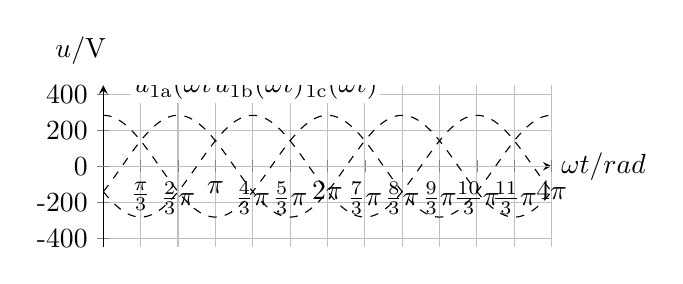
\begin{tikzpicture}
               \begin{axis}[
                   % x/y range adjustment
                   xmin=0, xmax=720,
                   ymin=-450, ymax=450,
                   samples=500,
                   axis y line=center,
                   axis x line=middle,
                   extra y ticks=0,
                   % Label text
                   xlabel={$\omega t / \text{rad}$},,
                   ylabel={$u/\mathrm{V}$},
                   % Label adjustment
                   x label style={at={(axis description cs:1,0.5)},anchor=west},
                   y label style={at={(axis description cs:-.05,.97)},anchor=south,yshift=0.2cm},
                   width=0.6\textwidth,
                   height=0.3\textwidth,
                   % x-Ticks
                   xtick={0,60,120,180,240,300,360, 420, 480, 540, 600, 660, 720},
                   xticklabels={,$\frac{\pi}{3}$,$\frac{2}{3}\pi$,$\pi$, $\frac{4}{3}\pi$,$\frac{5}{3}\pi$,$2\pi$, $\frac{7}{3}\pi$, $\frac{8}{3}\pi$,$\frac{9}{3}\pi$,$\frac{10}{3}\pi$,$\frac{11}{3}\pi$,$4\pi$},
                   xticklabel style = {anchor=north},
                   % y-Ticks
                   ytick={400,200,0,-200,-400},
                   yticklabels={400,200,0,-200,-400},
                   yticklabel style = {anchor=east},
                   % Grid layout
                   grid,
                   %grid style={line width=.1pt, draw=gray!10},
                   %major grid style={line width=.2pt,draw=gray!90},
                     ]
               % Voltage u1a(wt), u1b(wt) u1c(wt)
               \addplot[black, domain= 0:720,dashed] {282.84*cos(x)};
               \addplot[black, domain= 0:720,dashed] {282.84*cos(x+120)};
               \addplot[black, domain= 0:720,dashed] {282.84*cos(x+240)};
               % Label of u1c
               \node[black, fill=white, inner sep = 1pt, anchor = south] at (axis cs:370,350) {$u_{\mathrm{1c}}(\omega t)$}; 
               % Label of u1a
               \node[black, fill=white, inner sep = 1pt, anchor = south] at (axis cs:120,350) {$u_{\mathrm{1a}}(\omega t)$};           
               % Label of u1b
               \node[black, fill=white, inner sep = 1pt, anchor = south] at (axis cs:250,350) {$u_{\mathrm{1b}}(\omega t)$};

           \end{axis}     
           \end{tikzpicture}
           \caption{Output voltage $u_\mathrm{2}(t)$ for $\alpha$.}
           \label{fig:Task03_M3C_with_RLE}
   \end{figure}